% Disease Spread Modeling Using Dynamic Bayesian Networks
% Compile: pdflatex PGM_Project_Presentation.tex  (run twice for TOC)
\documentclass[aspectratio=169,11pt]{beamer}

\usetheme{Madrid}
\usecolortheme{default}
\setbeamertemplate{navigation symbols}{}
\setbeamertemplate{footline}[frame number]

\usepackage{graphicx}
\usepackage{booktabs}
\usepackage{amsmath,amssymb}
\usepackage{tikz}
\usetikzlibrary{arrows.meta,positioning,shapes}

\graphicspath{{../outputs/notebook/}}

\title{Disease Spread Modeling Using\\Dynamic Bayesian Networks}
\subtitle{Probabilistic Graphical Models --- Project Presentation}
\author{Your Name}
\institute{Course Project}
\date{\today}

\begin{document}

%----------------------------------------------------------------------
\begin{frame}
  \titlepage
\end{frame}

%----------------------------------------------------------------------
\begin{frame}{Outline}
  \tableofcontents
\end{frame}

%======================================================================
\section{Introduction}
%======================================================================

\begin{frame}{Motivation}
  \begin{itemize}
    \item Infectious diseases spread through \textbf{contact networks} over \textbf{time}.
    \item Health authorities observe \textbf{tests and symptoms}, not full infection states.
    \item We need a principled framework to answer:
  \end{itemize}
  \vspace{0.6em}
  \begin{block}{Central query}
    Given symptom/test observations across a population, what is the
    \textbf{probability that a given individual is currently infected}?
  \end{block}
\end{frame}

\begin{frame}{Project objectives}
  Model temporal disease spread with a \textbf{Dynamic Bayesian Network (DBN)}:
  \begin{itemize}
    \item \textbf{Latent variables:} SEIR states per person per day\\
          Susceptible, Exposed, \textbf{Infected}, Recovered
    \item \textbf{Observations:} reported test results (positive / negative / missing)
    \item \textbf{Data:} real-world COVID-19 contact tracing (Geneva, 2020)
  \end{itemize}
  \vspace{0.5em}
  Cover the three core pillars of Probabilistic Graphical Models:
  \begin{enumerate}
    \item Representation \quad 2.\ Inference \quad 3.\ Learning
  \end{enumerate}
\end{frame}

%======================================================================
\section{Data \& Preprocessing}
%======================================================================

\begin{frame}{Epidemic data}
  \begin{columns}[T]
    \column{0.52\textwidth}
    \textbf{Source:} Geneva COVID-19 contact tracing (GEgraph)
    \begin{itemize}
      \item Individual PCR test dates
      \item Documented close contacts
      \item National context: OWID Switzerland
    \end{itemize}
    \vspace{0.5em}
    \textbf{Preprocessing pipeline}
    \begin{enumerate}
      \item Extract connected contact subgraph
      \item Align calendar days to time slices
      \item Build observation matrix $Y_{t,i}$
    \end{enumerate}
    \column{0.46\textwidth}
    \centering
    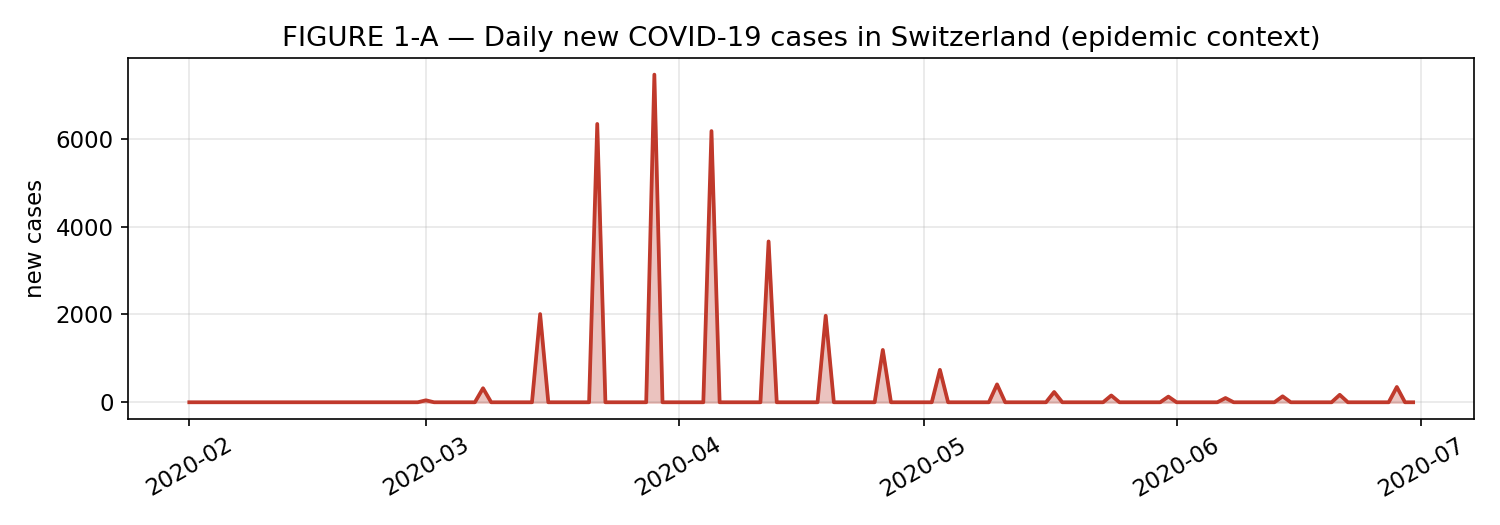
\includegraphics[width=\linewidth]{fig1a_epidemic_context.png}
    \vspace{-0.3em}
    {\footnotesize Daily new cases in Switzerland (context)}
  \end{columns}
\end{frame}

\begin{frame}{Dataset summary}
  \begin{table}
    \centering
    \begin{tabular}{@{}ll@{}}
      \toprule
      \textbf{Quantity} & \textbf{Value} \\
      \midrule
      Individuals (nodes) & 31 \\
      Contact edges & 49 \\
      Average degree & 3.16 \\
      Time period & 10 Mar -- 31 Aug 2020 \\
      Time steps & 175 days \\
      Positive tests observed & 11 \\
      Missing observations & $\approx$99.8\% \\
      \bottomrule
    \end{tabular}
  \end{table}
  \vspace{0.5em}
  Observations are \textbf{sparse}: most person-days have no test record.
  The DBN must infer latent SEIR states from limited evidence.
\end{frame}

\begin{frame}{Contact network \& observations}
  \begin{columns}[T]
    \column{0.48\textwidth}
    \centering
    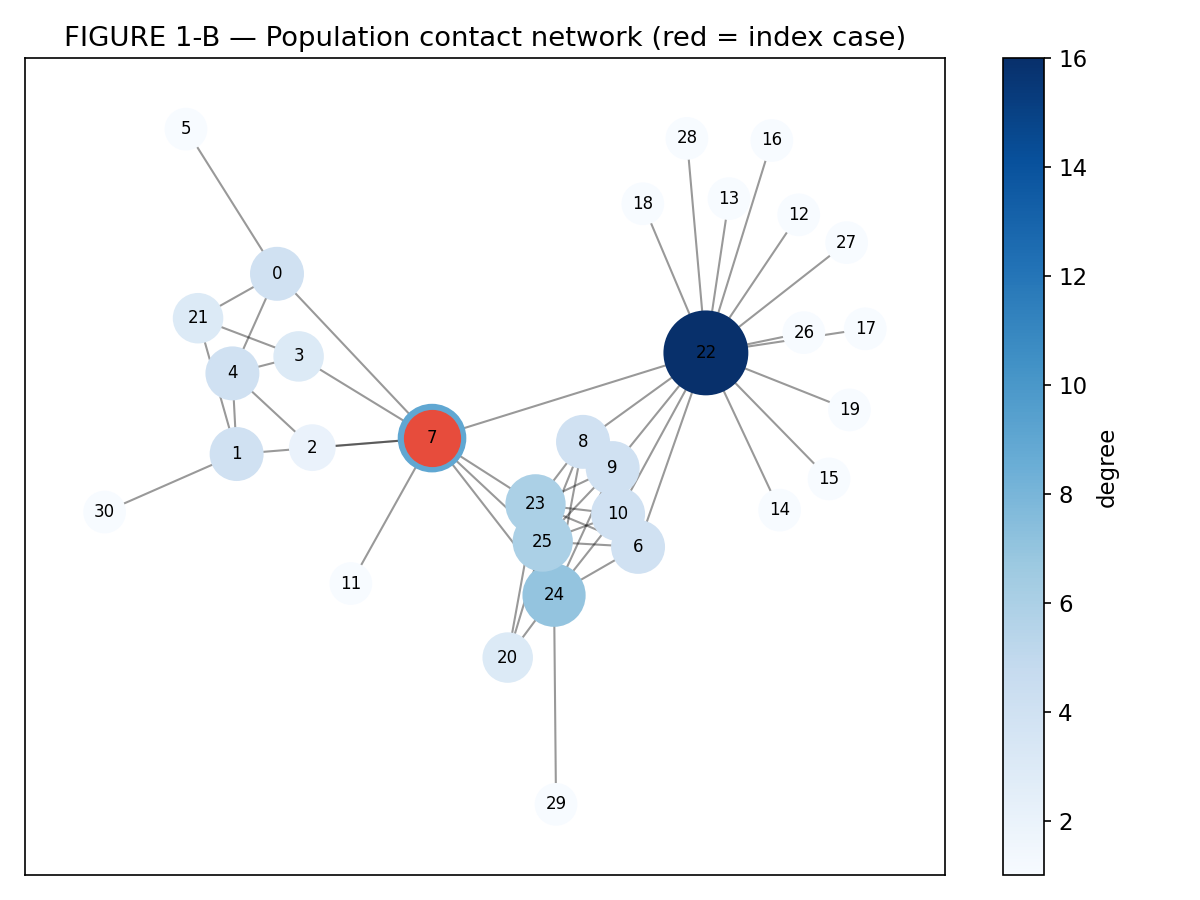
\includegraphics[width=\linewidth]{fig1b_network.png}
    {\footnotesize Contact network (red = index case)}
    \column{0.48\textwidth}
    \centering
    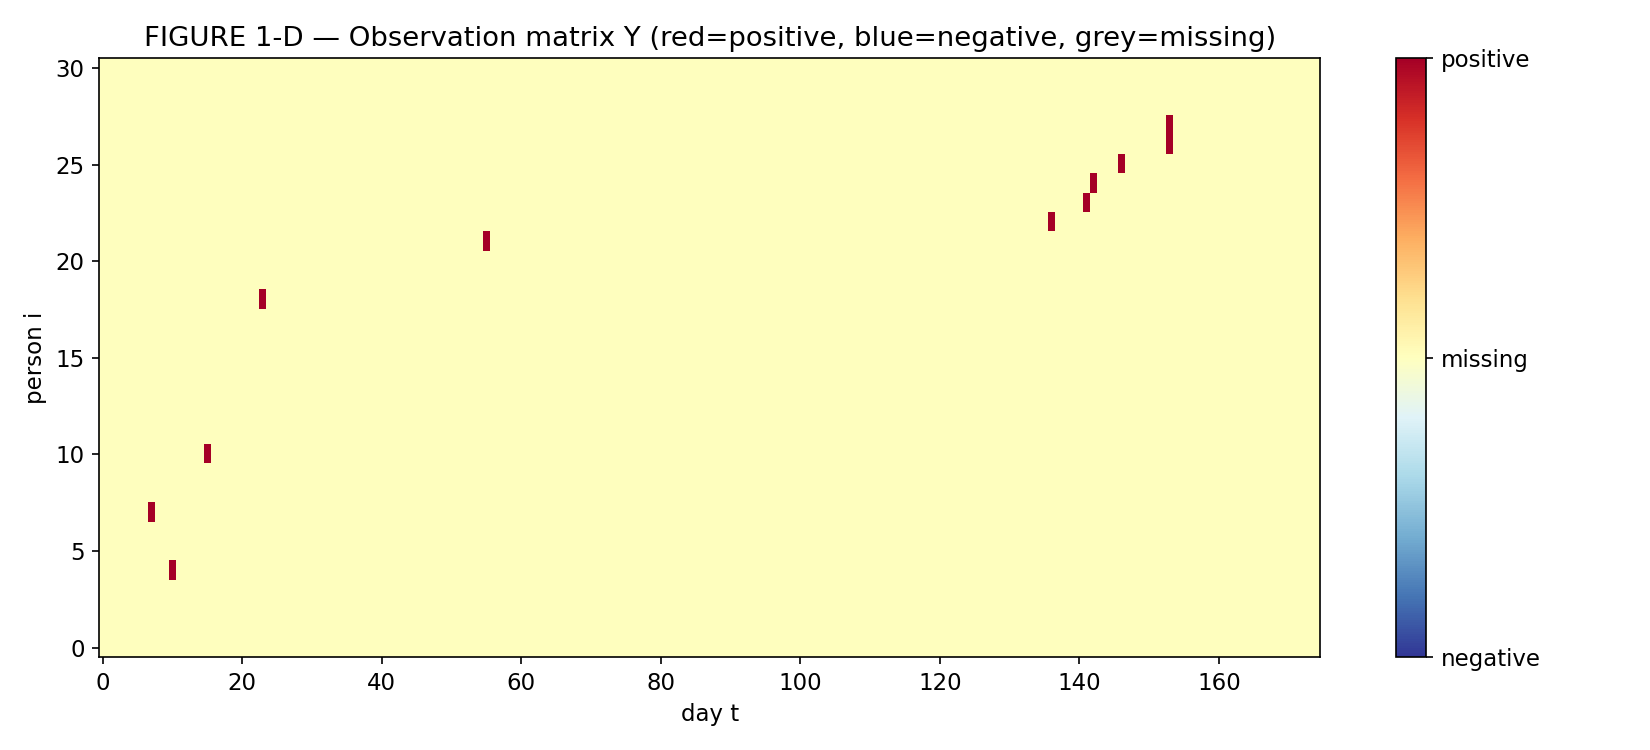
\includegraphics[width=\linewidth]{fig1d_observations.png}
    {\footnotesize Observation matrix $Y$ (red = positive test)}
  \end{columns}
\end{frame}

%======================================================================
\section{Representation}
%======================================================================

\begin{frame}{SEIR latent states}
  \begin{columns}[T]
    \column{0.55\textwidth}
    Each person $i$ at time $t$ has latent state $X_i^t \in \{S,E,I,R\}$:
    \begin{itemize}
      \item $S$ --- Susceptible
      \item $E$ --- Exposed (infected, not yet infectious)
      \item $I$ --- \textbf{Infected} (infectious)
      \item $R$ --- Recovered
    \end{itemize}
    \textbf{Parameters}
    \begin{itemize}
      \item $\beta$ --- transmission per infectious contact
      \item $\sigma$ --- rate $E \to I$
      \item $\gamma$ --- rate $I \to R$
    \end{itemize}
    \column{0.42\textwidth}
    \centering
    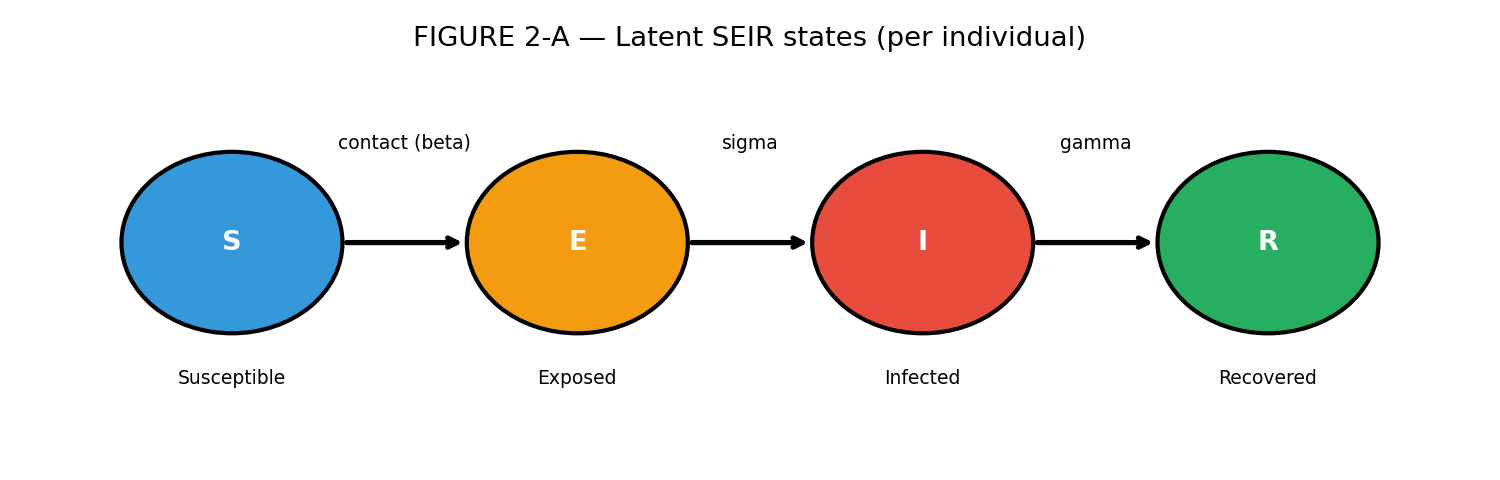
\includegraphics[width=\linewidth]{fig2a_seir.png}
    {\footnotesize SEIR compartment transitions}
  \end{columns}
\end{frame}

\begin{frame}{Dynamic Bayesian Network (2-time-slice)}
  \begin{columns}[T]
    \column{0.50\textwidth}
    \centering
    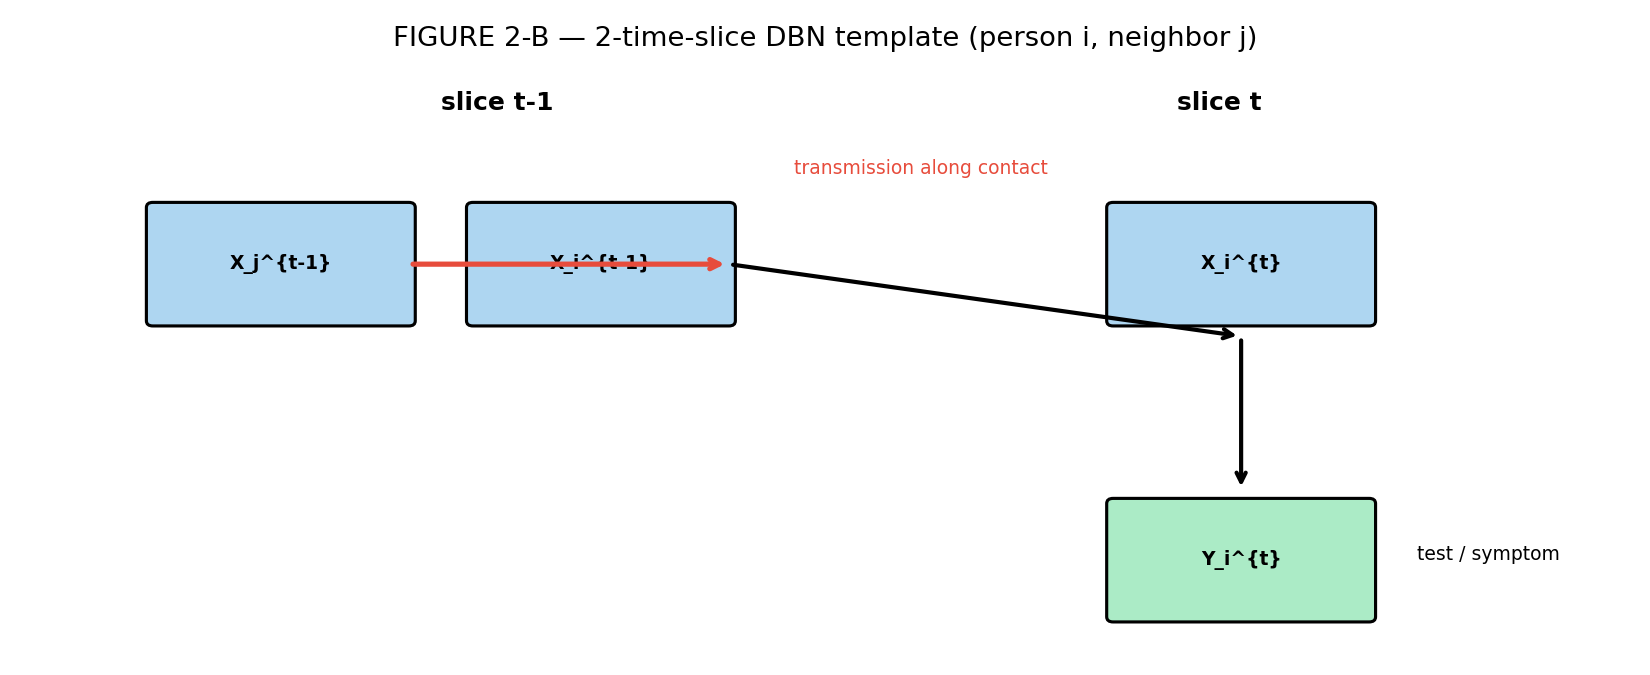
\includegraphics[width=\linewidth]{fig2b_dbn_plate.png}
    {\footnotesize 2-time-slice template}
    \column{0.48\textwidth}
    \textbf{Intra-slice edges} (same day)
    \begin{itemize}
      \item $X_i^t \to Y_i^t$ \quad (test emission)
    \end{itemize}
    \textbf{Inter-slice edges} (across days)
    \begin{itemize}
      \item $X_i^{t-1} \to X_i^t$ \quad (within-person dynamics)
      \item $X_j^{t-1} \to X_i^t$ \quad (transmission along contacts)
    \end{itemize}
    \vspace{0.4em}
  \end{columns}
\end{frame}

\begin{frame}{Observation model}
  Tests are noisy indicators of infection state:
  \begin{align*}
    P(Y_i^t = + \mid X_i^t = I) &= \text{sensitivity} = 0.90 \\
    P(Y_i^t = - \mid X_i^t \neq I) &= \text{specificity} = 0.95
  \end{align*}
  \begin{columns}[T]
    \column{0.48\textwidth}
    \centering
    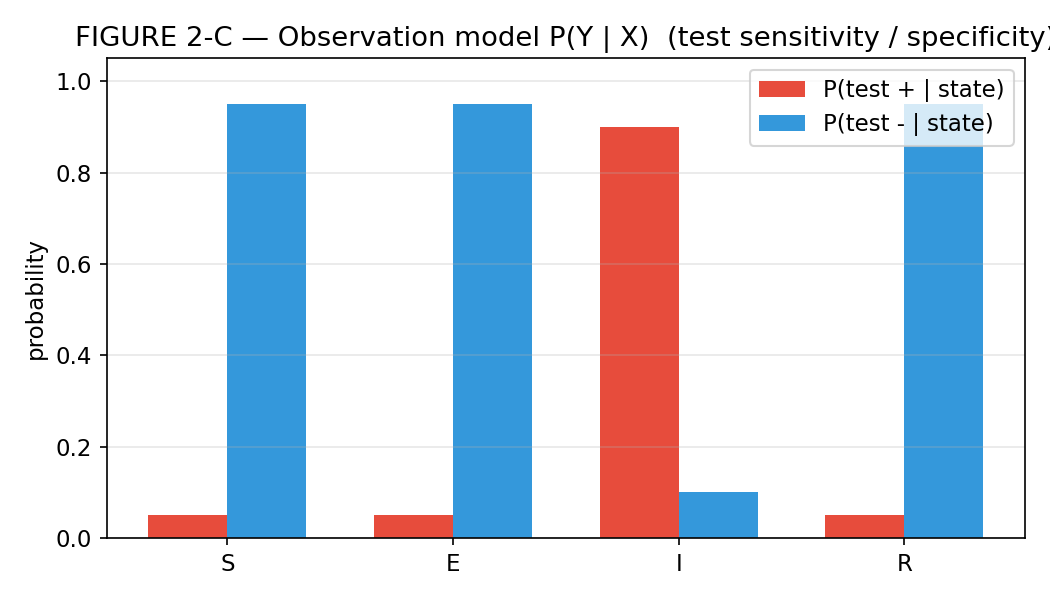
\includegraphics[width=\linewidth]{fig2c_emission.png}
    {\footnotesize Emission probabilities $P(Y \mid X)$}
    \column{0.48\textwidth}
    \centering
    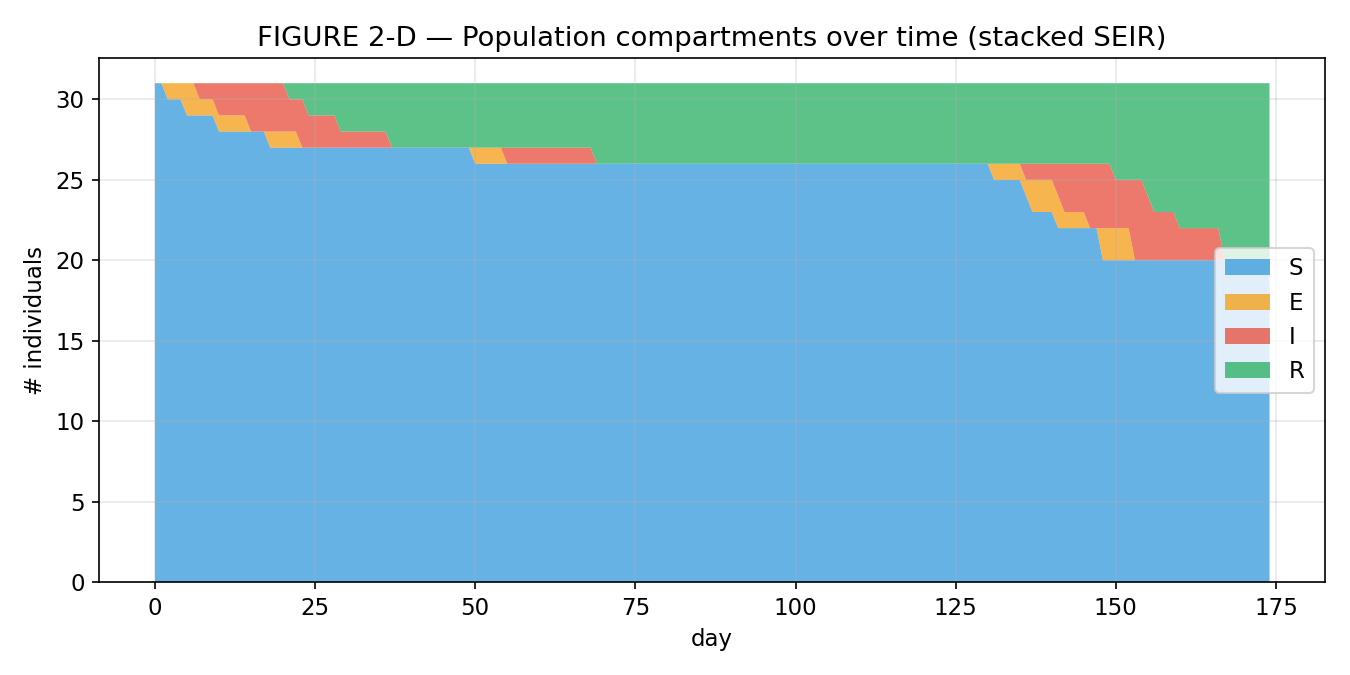
\includegraphics[width=\linewidth]{fig2d_seir_stack.png}
    {\footnotesize SEIR compartments over time}
  \end{columns}
\end{frame}

\begin{frame}{Graph structure}
  Spatial structure = \textbf{contact network} from tracing data.
  \begin{columns}[T]
    \column{0.48\textwidth}
    \centering
    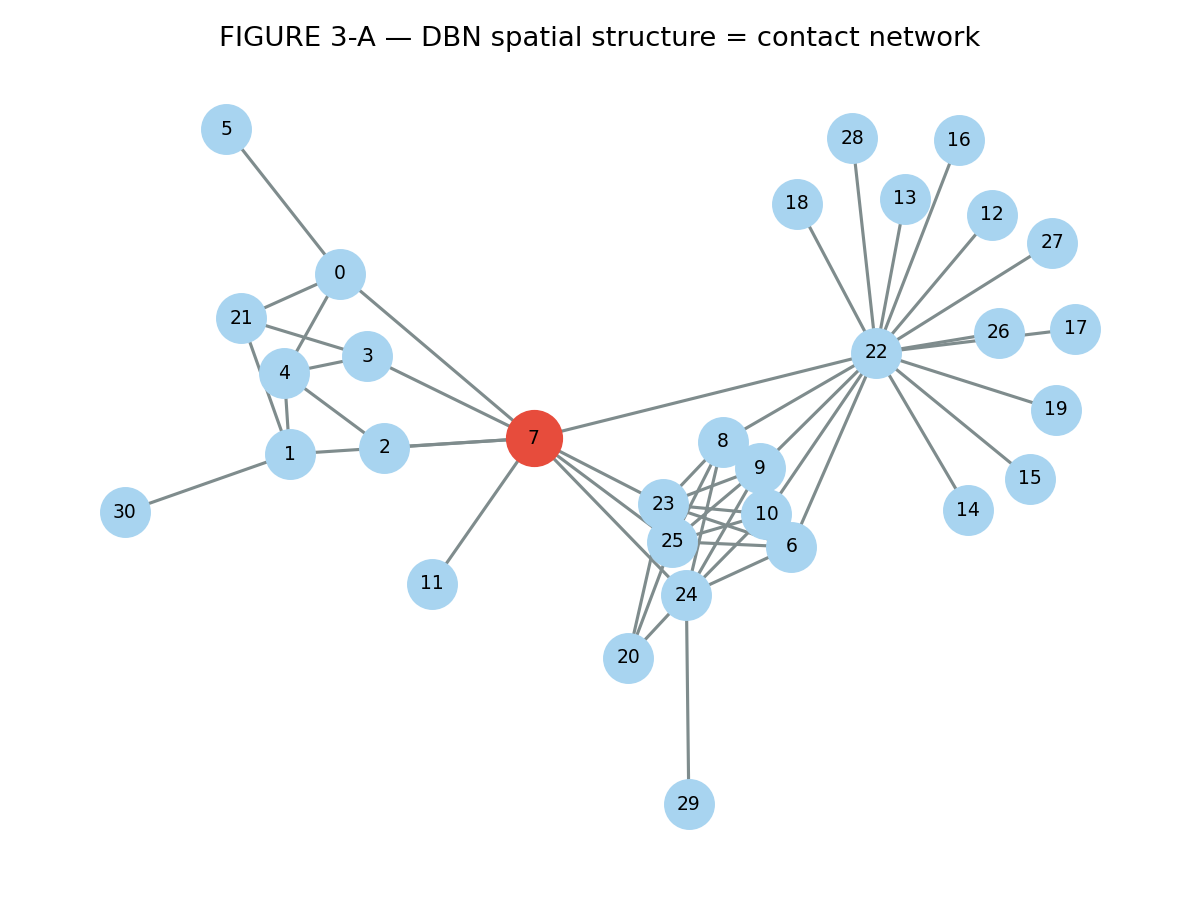
\includegraphics[width=\linewidth]{fig3a_structure.png}
    {\footnotesize DBN spatial structure}
    \column{0.48\textwidth}
    \centering
    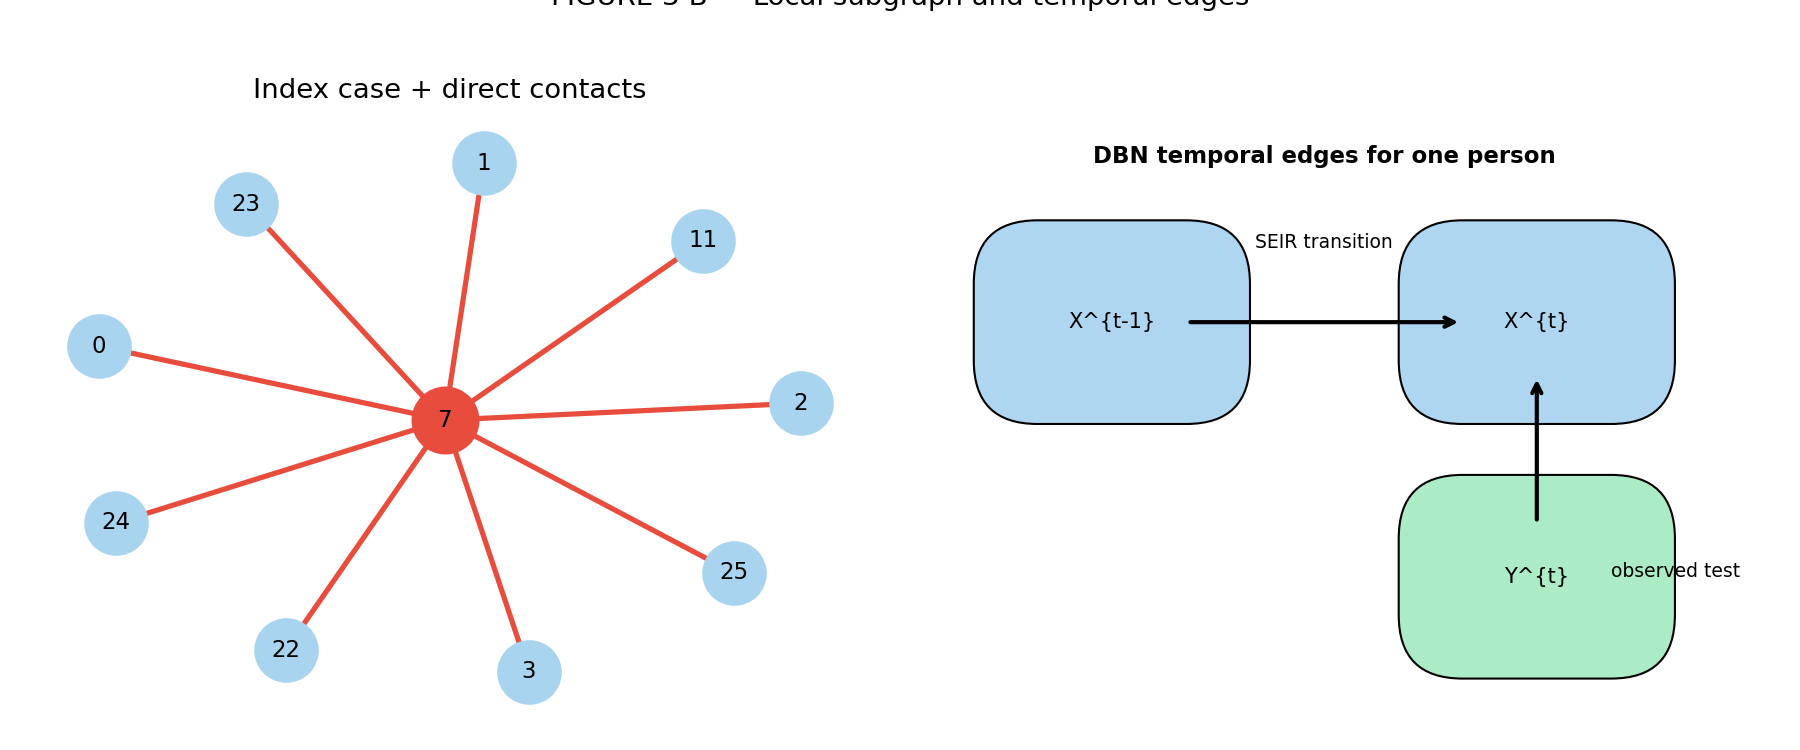
\includegraphics[width=\linewidth]{fig3b_local_dbn.png}
    {\footnotesize Local subgraph \& temporal edges}
  \end{columns}
\end{frame}

%======================================================================
\section{Learning}
%======================================================================

\begin{frame}{Parameter learning (EM algorithm)}
  SEIR states are \textbf{latent}; only tests are observed.
  \begin{block}{Expectation--Maximisation}
    \textbf{E-step:} forward--backward inference $\Rightarrow$ soft SEIR counts\\
    \textbf{M-step:} update $\beta$, $\sigma$, $\gamma$ from expected transitions
  \end{block}
  \begin{columns}[T]
    \column{0.48\textwidth}
    \centering
    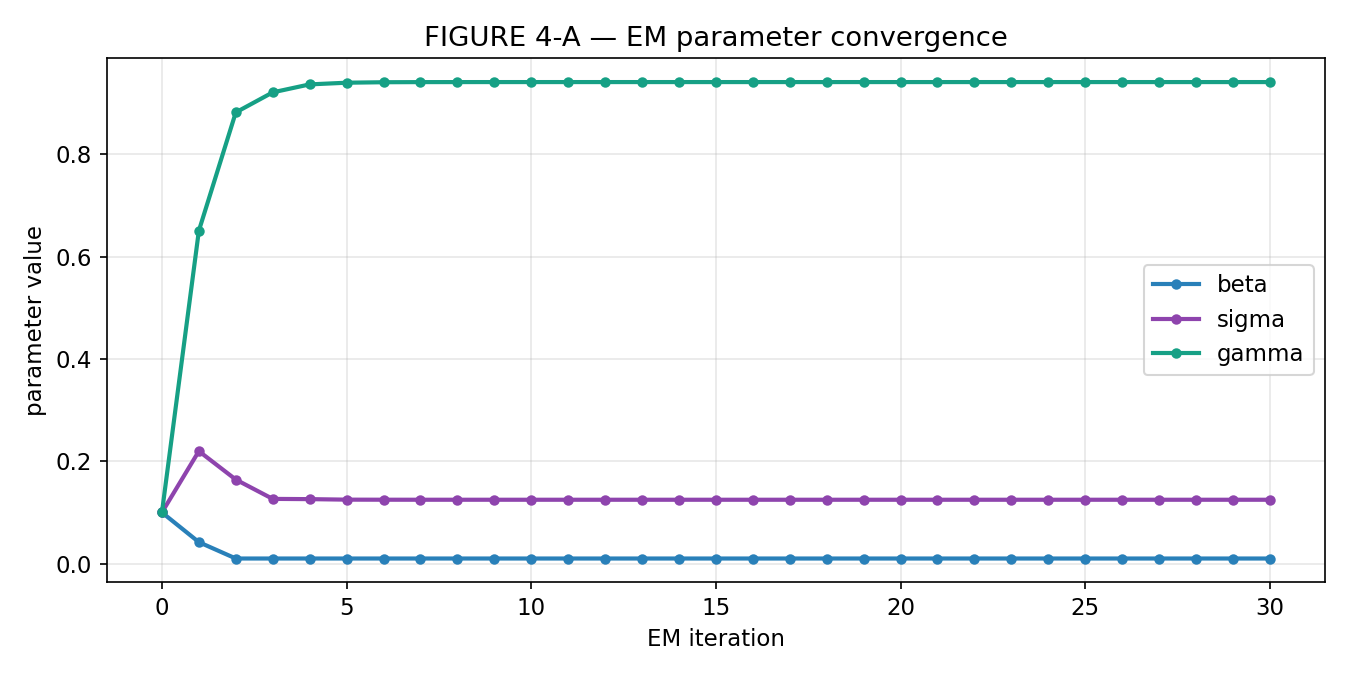
\includegraphics[width=\linewidth]{fig4a_em.png}
    {\footnotesize EM convergence (25 iterations)}
    \column{0.48\textwidth}
    \centering
    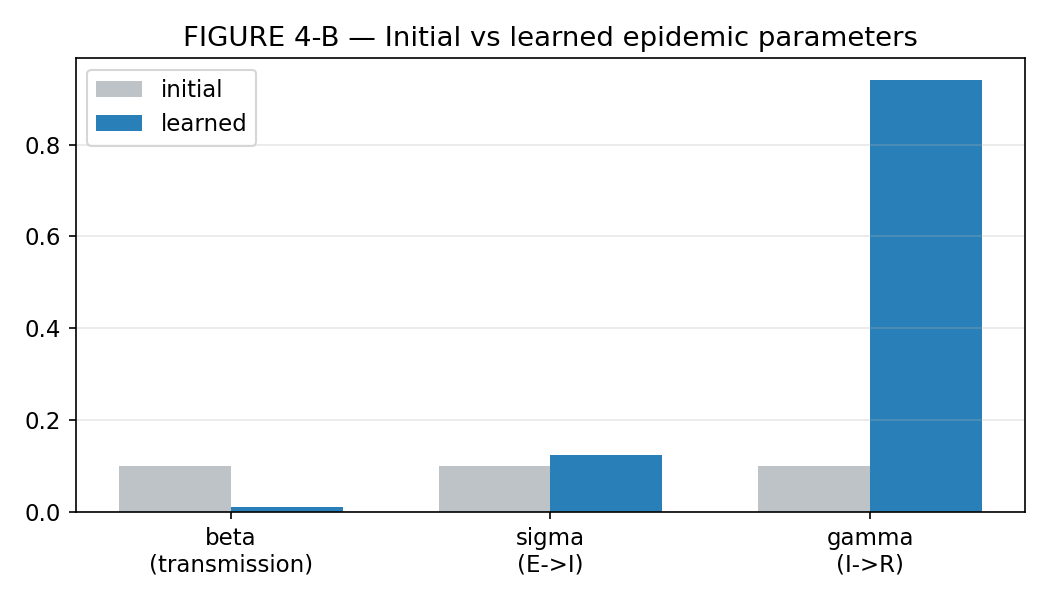
\includegraphics[width=\linewidth]{fig4b_params.png}
    {\footnotesize Initial vs.\ learned parameters}
  \end{columns}
\end{frame}

\begin{frame}{Learned parameters}
  \begin{table}
    \centering
    \begin{tabular}{@{}lccc@{}}
      \toprule
      \textbf{Parameter} & \textbf{Initial} & \textbf{Learned (EM)} & \textbf{Meaning} \\
      \midrule
      $\beta$  & 0.10 & 0.01  & transmission rate \\
      $\sigma$ & 0.10 & 0.125 & exposed $\to$ infected \\
      $\gamma$ & 0.10 & 0.941 & infected $\to$ recovered \\
      \bottomrule
    \end{tabular}
  \end{table}
  \vspace{0.4em}
  \begin{columns}[T]
    \column{0.55\textwidth}
    \small
    High $\gamma$ and low $\beta$ are consistent with \textbf{sparse positive tests}
    and short infectious episodes in the subgraph.
    \column{0.42\textwidth}
    \centering
    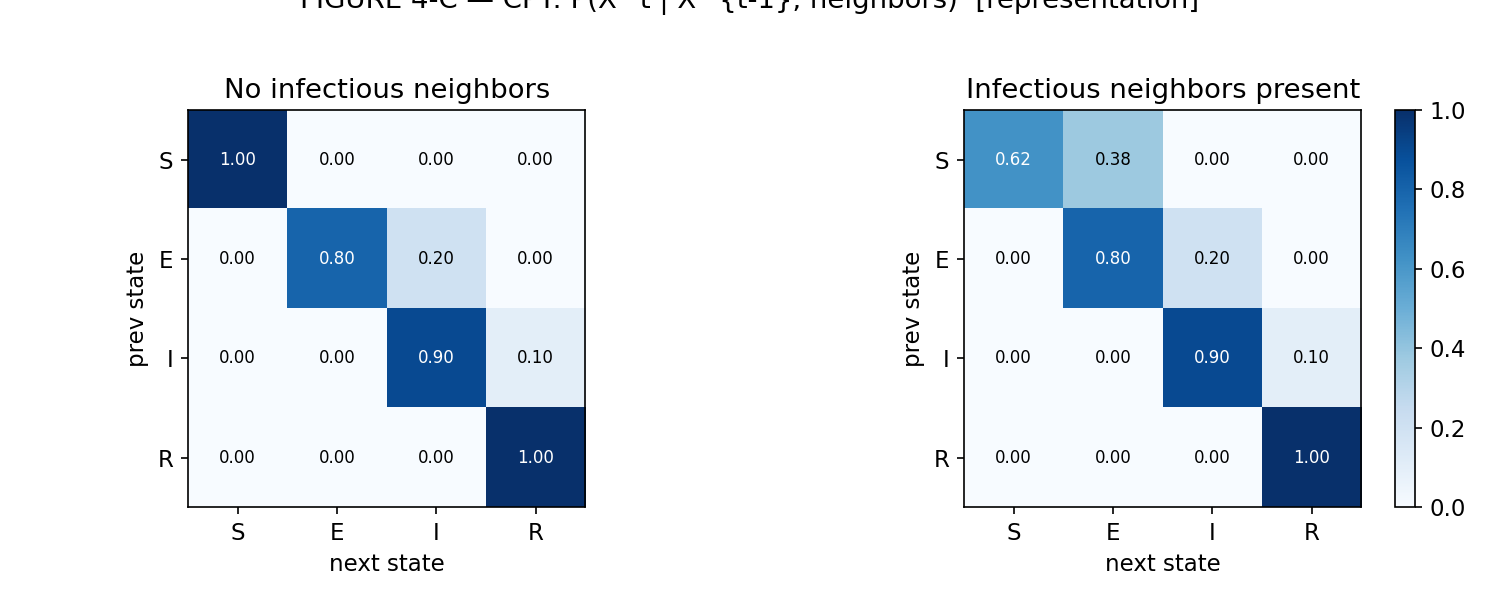
\includegraphics[width=\linewidth]{fig4c_cpt.png}
    {\footnotesize Example transition CPTs}
  \end{columns}
\end{frame}

%======================================================================
\section{Inference}
%======================================================================

\begin{frame}{Inference methods}
  \textbf{Pillar 2 --- Inference:} answer queries on latent infection states.
  \begin{itemize}
    \item \textbf{Variable elimination} --- single-person test model (pgmpy)
    \item \textbf{Forward--backward belief propagation} --- full temporal DBN on network
  \end{itemize}
  \begin{columns}[T]
    \column{0.48\textwidth}
    \centering
    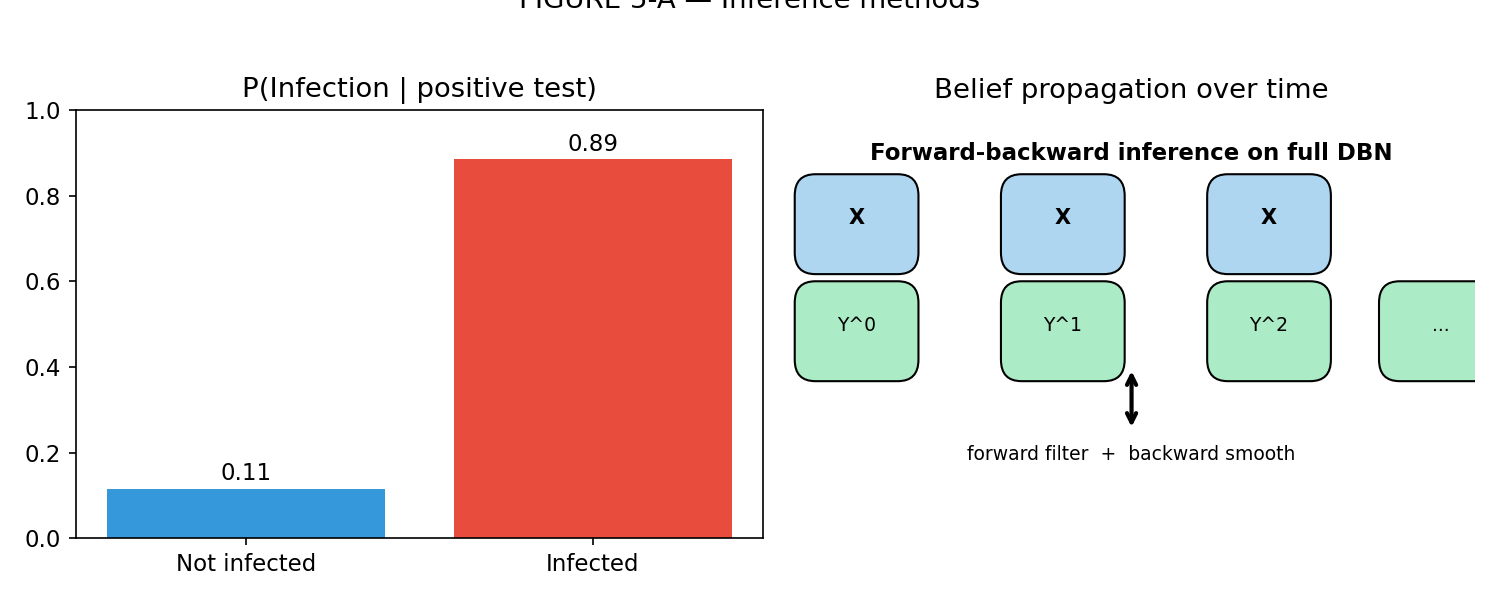
\includegraphics[width=\linewidth]{fig5a_inference.png}
    {\footnotesize VE demo \& belief propagation schematic}
    \column{0.48\textwidth}
    \textbf{Example query}
    \begin{itemize}
      \item Index case, day 10:\\
            $P(I \mid Y) \approx 0.01$
      \item Max posterior over network:\\
            $\max_{t,i} P(X_i^t{=}I \mid Y) \approx 0.48$
    \end{itemize}
  \end{columns}
\end{frame}

\begin{frame}{Posterior: $P(\text{Infected} \mid \text{all tests})$}
  \begin{columns}[T]
    \column{0.55\textwidth}
    \centering
    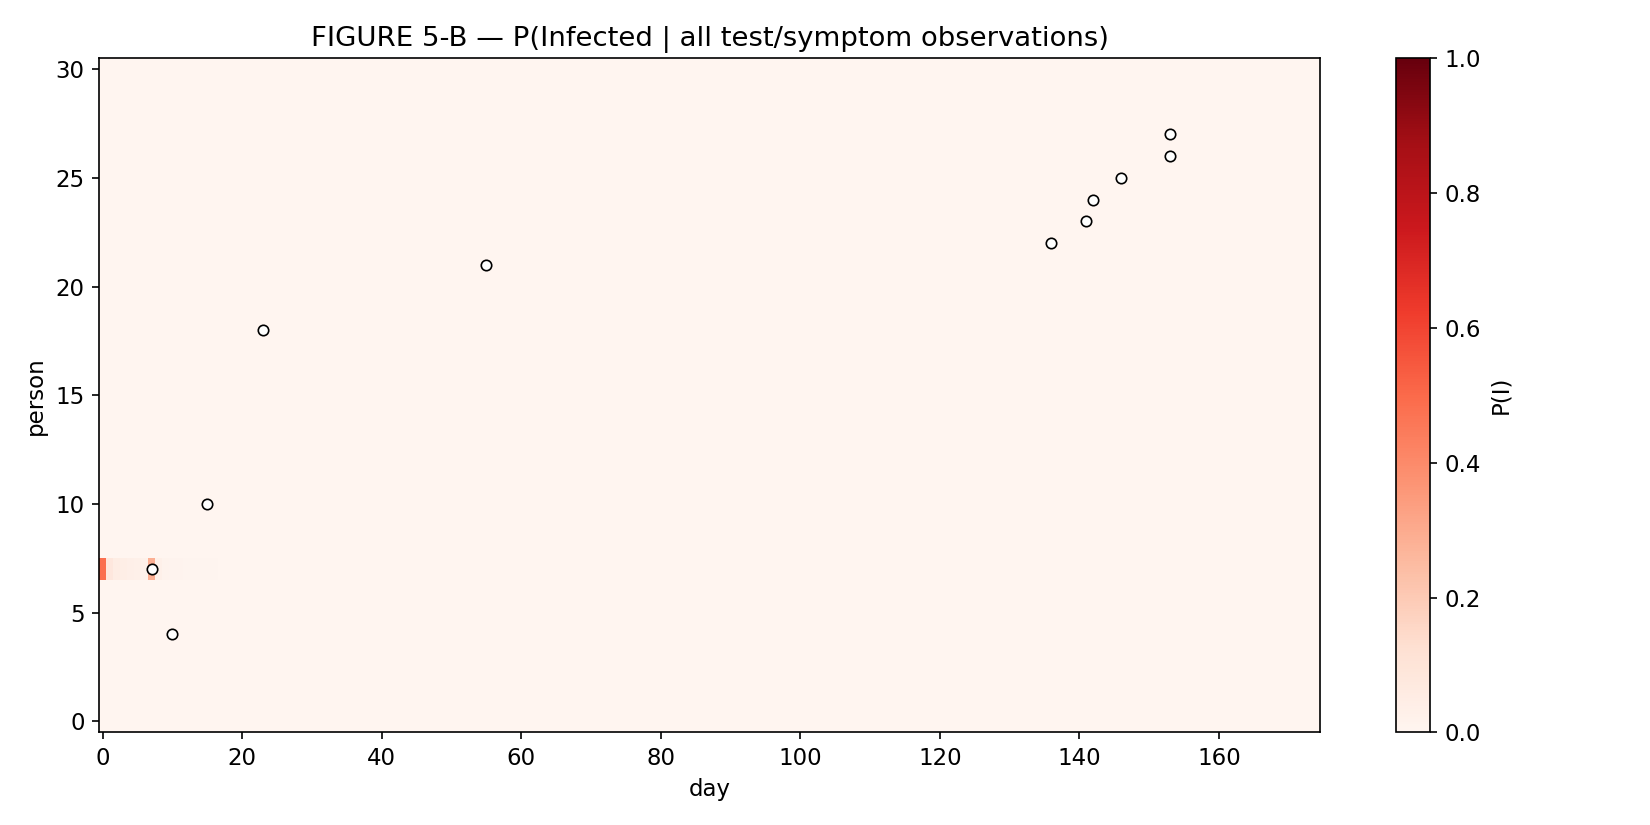
\includegraphics[width=\linewidth]{fig5b_heatmap.png}
    {\footnotesize Posterior heatmap (white dots = positive tests)}
    \column{0.42\textwidth}
    \centering
    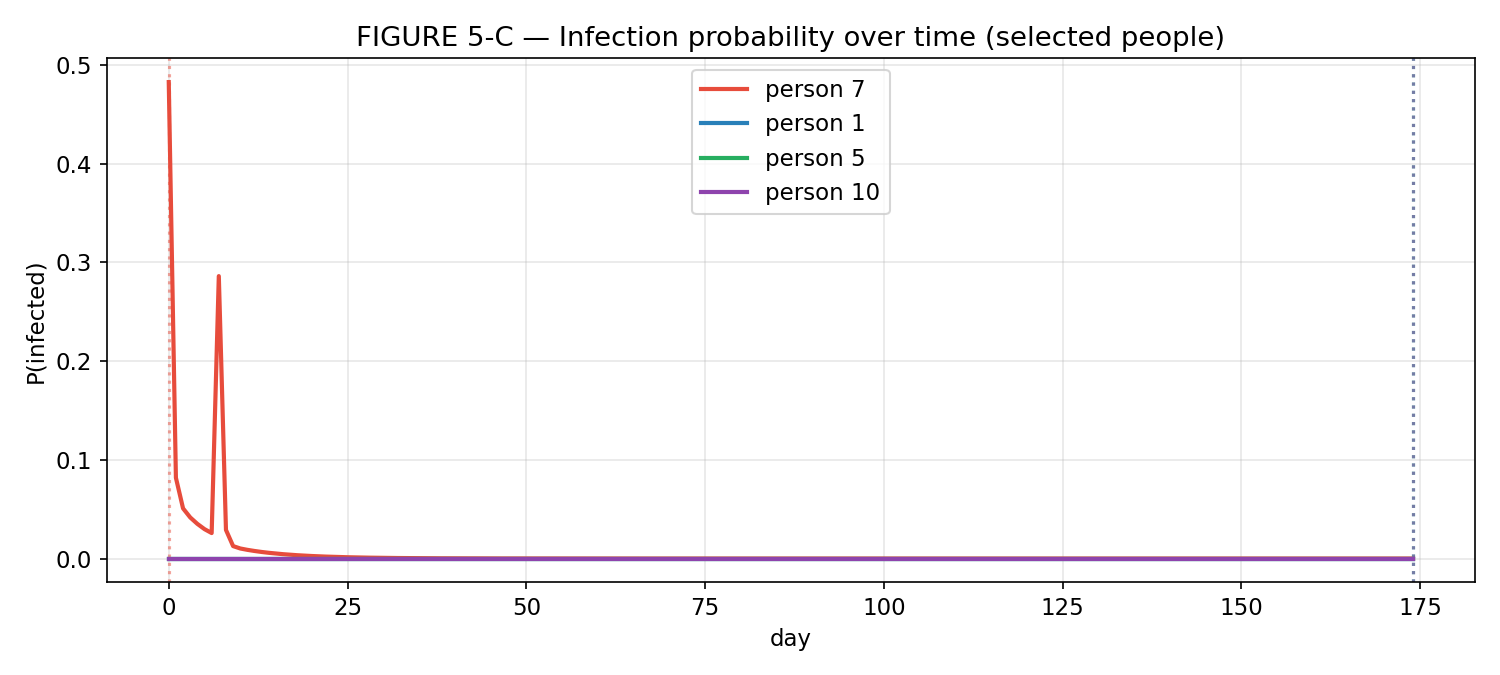
\includegraphics[width=\linewidth]{fig5c_timeseries.png}
    {\footnotesize $P(I)$ over time (selected people)}
  \end{columns}
\end{frame}

\begin{frame}{Network-level posterior}
  \begin{columns}[T]
    \column{0.48\textwidth}
    \centering
    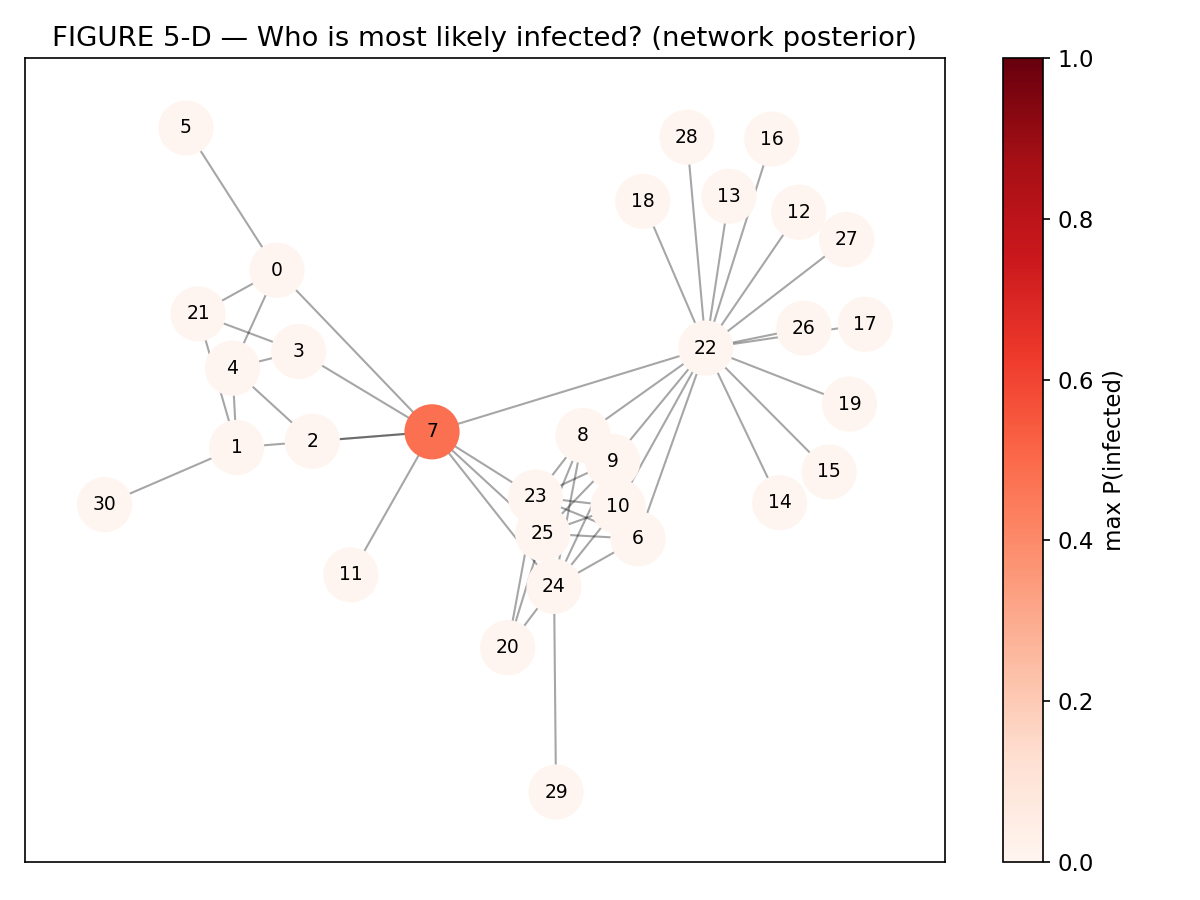
\includegraphics[width=\linewidth]{fig5d_network.png}
    {\footnotesize Nodes coloured by $\max_t P(X_i^t{=}I \mid Y)$}
    \column{0.48\textwidth}
    \centering
    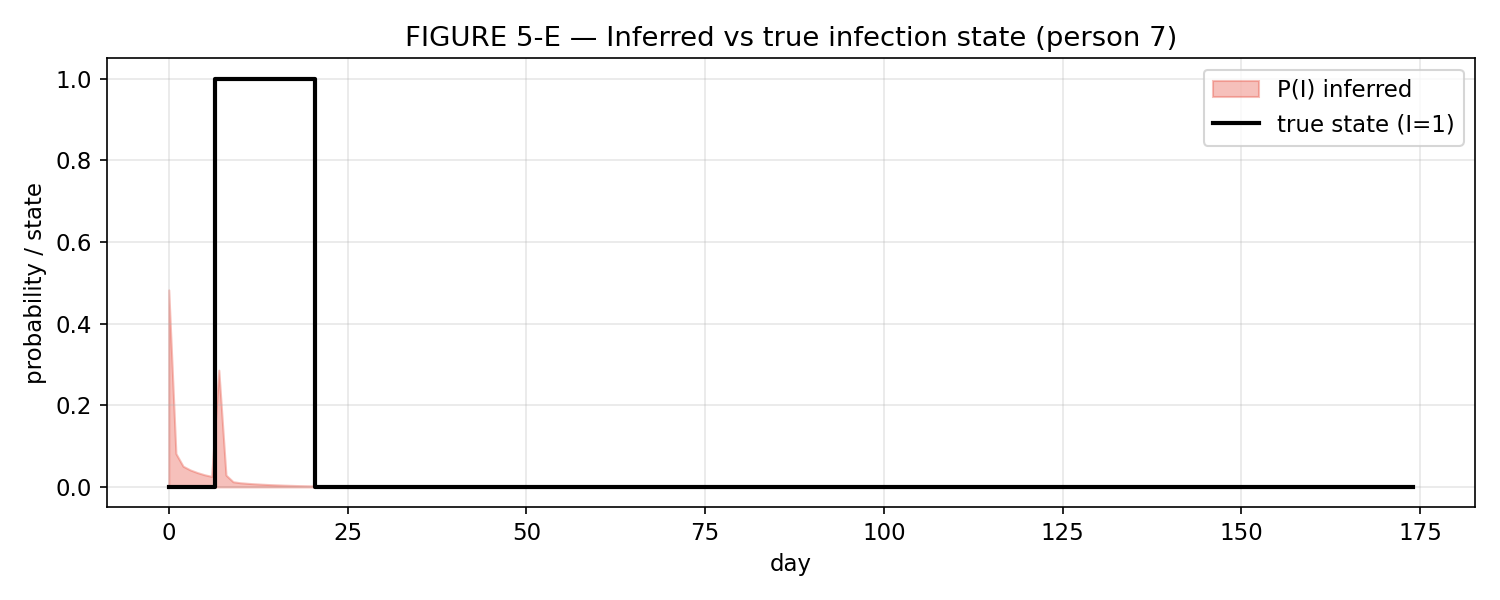
\includegraphics[width=\linewidth]{fig5e_compare.png}
    {\footnotesize Inferred vs.\ true state (index case)}
  \end{columns}
  \vspace{0.3em}
  \small Peak infected count in subgraph labels: 5 individuals.
\end{frame}

%======================================================================
\section{Evaluation \& Results}
%======================================================================

\begin{frame}{Evaluation dashboard}
  \centering
  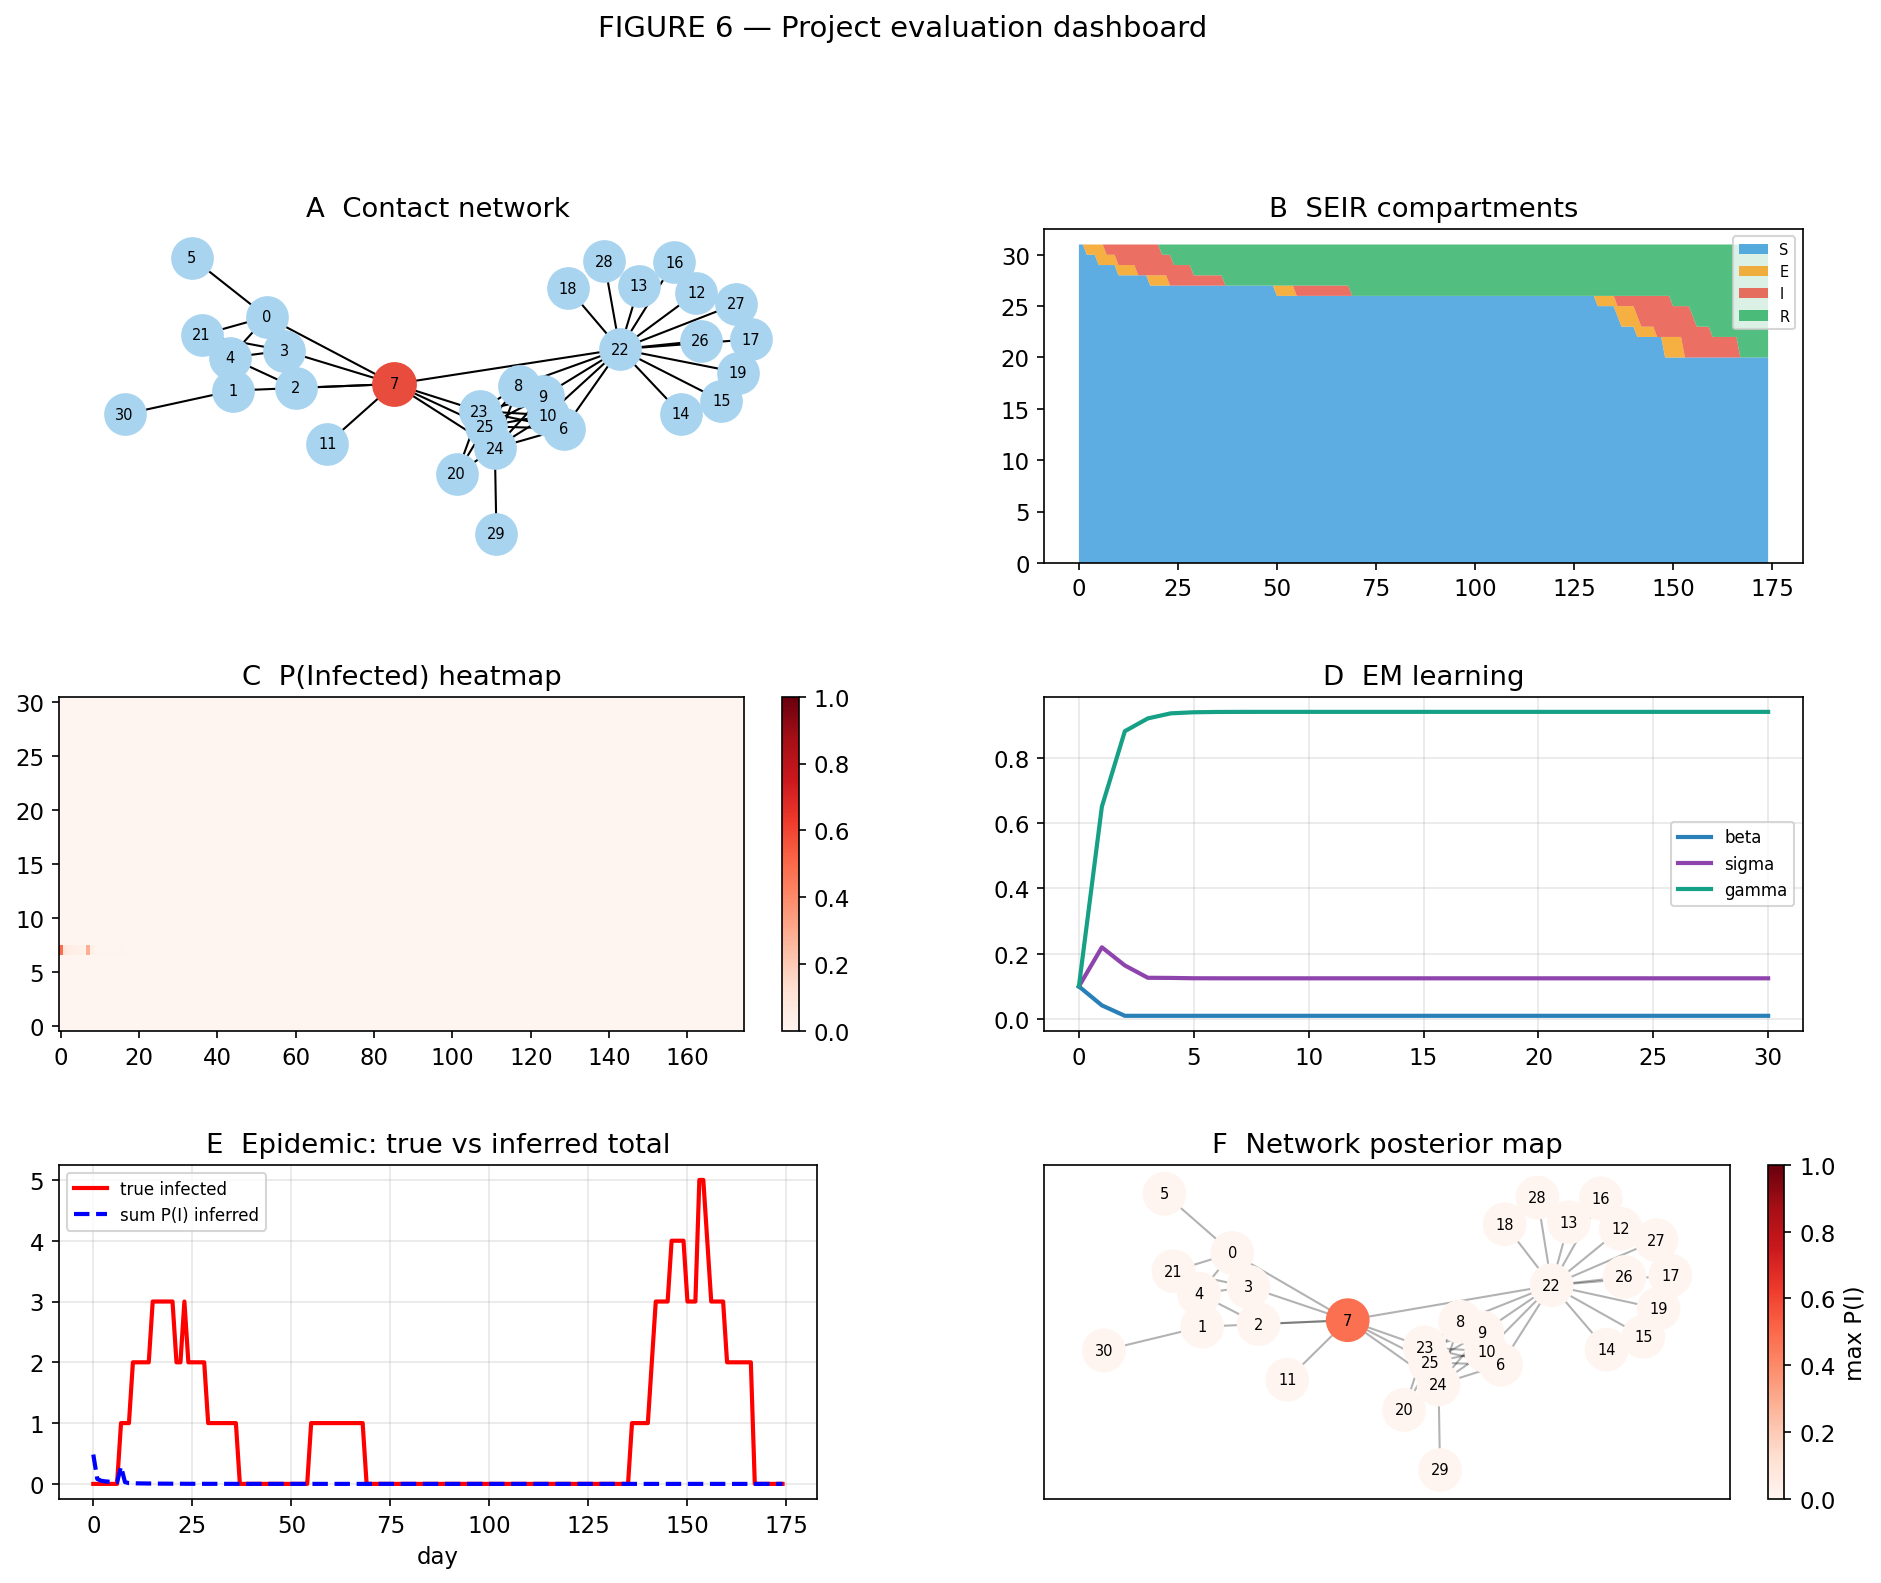
\includegraphics[width=0.92\linewidth]{fig6_dashboard.png}
  \vspace{0.2em}
  {\footnotesize Contact network, SEIR dynamics, posterior heatmap, EM learning, epidemic comparison}
\end{frame}

\begin{frame}{Key results}
  \begin{table}
    \centering
    \small
    \begin{tabular}{@{}p{5.2cm}p{5.8cm}@{}}
      \toprule
      \textbf{Result} & \textbf{Finding} \\
      \midrule
      Representation & 31-node contact network; 2-slice SEIR DBN with 124 pgmpy variables \\
      Data sparsity & 11 positive tests over 5{,}425 person-days ($\approx$0.2\%) \\
      Learning (EM) & $\beta{=}0.01$, $\sigma{=}0.13$, $\gamma{=}0.94$ after 25 iterations \\
      Inference & Posterior identifies high-risk individuals and time windows \\
      Main query & $P(\text{node } i \text{ infected} \mid Y)$ computed for any $(i,t)$ \\
      \bottomrule
    \end{tabular}
  \end{table}
  \vspace{0.5em}
  \begin{block}{Outcome}
    A working DBN pipeline that integrates \textbf{representation}, \textbf{inference},
    and \textbf{learning} on real epidemic contact-tracing data.
  \end{block}
\end{frame}

%======================================================================
\section{Conclusion}
%======================================================================

\begin{frame}{Conclusion}
  \textbf{Contributions}
  \begin{itemize}
    \item End-to-end DBN for disease spread on a real contact network
    \item Latent SEIR states with noisy test observations
    \item EM parameter estimation under partial observability
    \item Belief propagation answering infection-probability queries
  \end{itemize}
  \vspace{0.4em}
  \textbf{Limitations \& extensions}
  \begin{itemize}
    \item Very sparse tests $\Rightarrow$ uncertain posteriors; more data or synthetic validation helps
    \item Mean-field inference for scalability; exact DBN inference on small subgraphs
    \item Compare topology sensitivity (ER, WS, BA) and intervention scenarios
  \end{itemize}
\end{frame}

\begin{frame}
  \centering
  \Large Thank you
  \vspace{1em}

  \normalsize
  \textbf{Repository:} \texttt{notebooks/PGM\_EndToEnd\_Pipeline.ipynb}\\[0.4em]
  \textbf{Query answered:}\\
  $P(X_i^t = \text{Infected} \mid \{Y_{j,s}\}_{\text{all } j,s})$
  \vspace{1em}

  \small Questions?
\end{frame}

\end{document}
